\documentclass[9pt]{IEEEtran}

\usepackage[english]{babel}
\usepackage{graphicx}
\usepackage{epstopdf}
\usepackage{fancyhdr}
\usepackage{amsmath}
\usepackage{amsthm}
\usepackage{amssymb}
\usepackage{url}
\usepackage{array}
\usepackage{textcomp}
\usepackage{listings}
\usepackage{hyperref}
\usepackage{xcolor}
\usepackage{colortbl}
\usepackage{float}
\usepackage{gensymb}
\usepackage{longtable}
\usepackage{supertabular}
\usepackage{multicol}
\usepackage[justification=centering]{caption}
\usepackage[utf8x]{inputenc}

\usepackage[T1]{fontenc}
\usepackage{lmodern}
\input{glyphtounicode}
\pdfgentounicode=1

\graphicspath{{./figures/}}
\DeclareGraphicsExtensions{.pdf,.png,.jpg,.eps}

% correct bad hyphenation here
\hyphenation{op-tical net-works semi-conduc-tor trig-gs}

% ============================================================================================

\title{\vspace{0ex}
Lucas-Kanade and Horn-Schunck Optical Flow implementation and analysis}

\author{Aljaž Konec, 63190019\vspace{-4.0ex}}

% ============================================================================================

\begin{document}

\maketitle

\section{Introduction}
In this report we present the implementation and analysis of two optical flow methods: Lucas-Kanade and Horn-Schunck.
Both methods use derivatives of the image to estimate the motion between two frames.
Estimating motion in the image is important for many computer vision tasks such as object tracking, video stabilization, 3D reconstruction and surveillance.
Both methods are based on the use of derivatives in a small neighborhood of the image to estimate the motion of the pixels.
While the Lucas-Kanade method estimates the motion of the pixels using least squares, the Horn-Schunck method minimizes the global energy of the flow field.
We use matrix operations and convolution to efficiently compute both methods.

\section{Experiments}

\subsection*{Synthetic example}
In Figure \ref{lk-hs-noise} we present the results of both methods on a random noise image that is rotated by 1 degree.
Pixels at the edge of the image move further than those in the center.
The Lucas-Kanade method assumes the motion is relatively small and for this reason it fails to estimate the motion of some edge pixels near the top of the image.
Horn-Schunck method, on the other hand, minimizes the global energy of the flow field and is able to better estimate the motion of those edge pixels.
\begin{figure}[H]
    \centering
    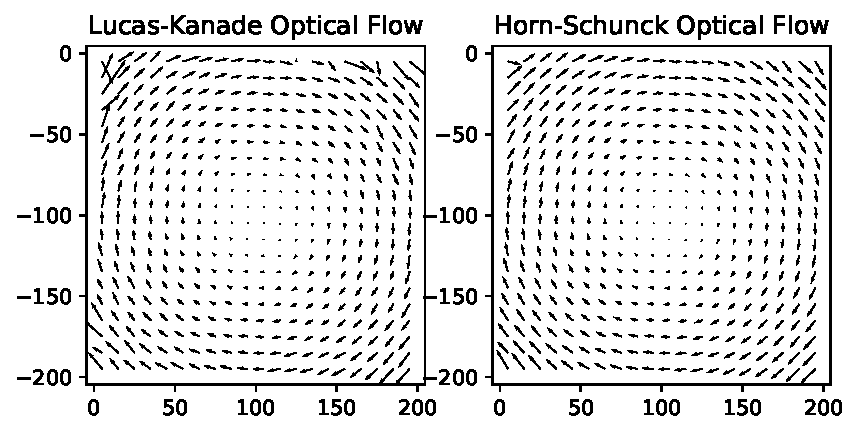
\includegraphics[width=0.5\textwidth]{LK_HS_noise.pdf}
    \vspace{-20px}
    \caption{Optical flow fields for Lucas-Kanade and Horn-Schunck methods on random noise.}
    \label{lk-hs-noise}
\end{figure}

\subsection*{Real world example}

Figure \ref{lk-hs-real} shows the results of both methods on 3 real world images.
In the first image (top row) Lucas-Kanade fails in the top right corner where there is a large flat surface with no texture which yields small gradients and thus creates a large error.
Horn-Schunck method somewhat negates these errors but they are still present.
In the second image (middle row) a similar occurence can be observed.
In the third image (bottom row) both methods fail to estimate the motion of the camera in the middle of the image as it is too large.
The lack of motion of the top right background is well estimated as the background is relatively textured and in the video we are approaching the camera stand which makes the motion very small.
\begin{figure}[H]
    \centering
    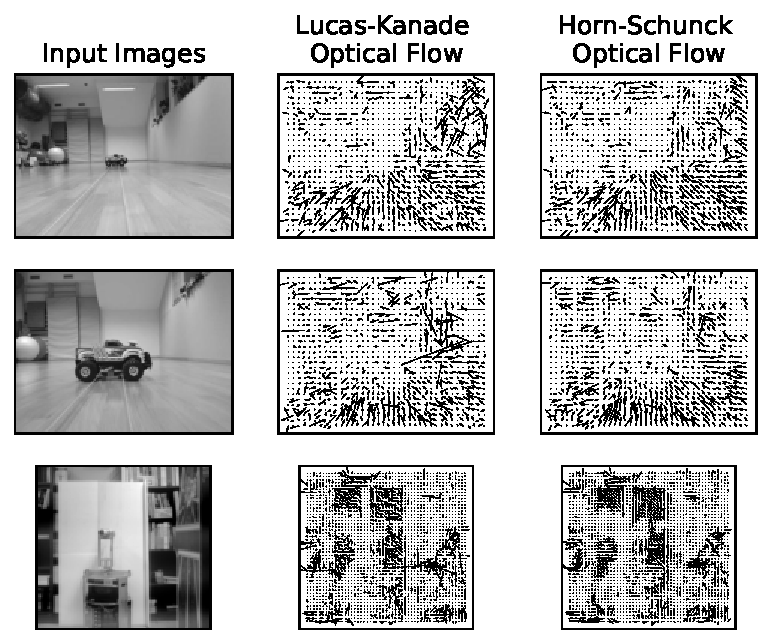
\includegraphics[width=0.5\textwidth]{LK_HS_real.pdf}
    \vspace{-15px}
    \caption{Optical flow fields for Lucas-Kanade and Horn-Schunck methods on a real world images.}
    \label{lk-hs-real}
\end{figure}

\subsection*{Lucas-Kanade with Harris corner response}
To better estimate the motion in the image we want to remove estimation on large homogeneous areas, i.e. areas with low gradients.
We use the Harris corner response to determine areas with edges and corners and only estimate the motion in those areas.
In Figure \ref{lk-improvement} we present the results of Lucas-Kanade method with Harris response.
Regions with low texture in the right side of the image (the wall and floor) have low absolute Harris response and as such their movement is not estimated.
\begin{figure}[H]
    \centering
    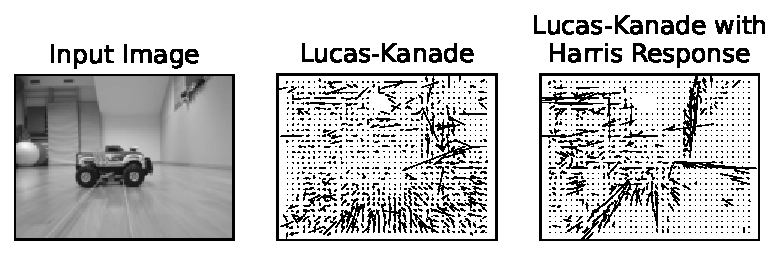
\includegraphics[width=0.5\textwidth]{LK_Harris.pdf}
    \vspace{-15px}
    \caption{Optical flow fields for Lucas-Kanade method with and without Harris corner response.}
    \label{lk-improvement}
\end{figure}

\subsection*{Parameter tuning}
For Lucas-Kanade method we can tune the size of the neighborhood window that is used to estimate the motion.
A larger window size provides more global information on the motion while a smaller window size provides more local information.
Typically a window size of 3x3 is used. In Figure \ref{lk-window} we present the results of Lucas-Kanade method with three different window sizes: 3x3, 7x7 and 15x15.
When approaching the car in the video, central pixels move less then edge pixels.
This small optical flow is detected by 3x3 and 7x7 window sizes.
At the same time these window sizes fail to detect the large optical flow occurring around the edges of the car.
The 15x15 window size is able to detect this large optical flow while also minimizing the noise in the center of the image where the motion is small.
In this case a larger size is a better solution, but in general the window size depends on whether we are interested in finding small or large motion in the image.
\begin{figure}[H]
    \centering
    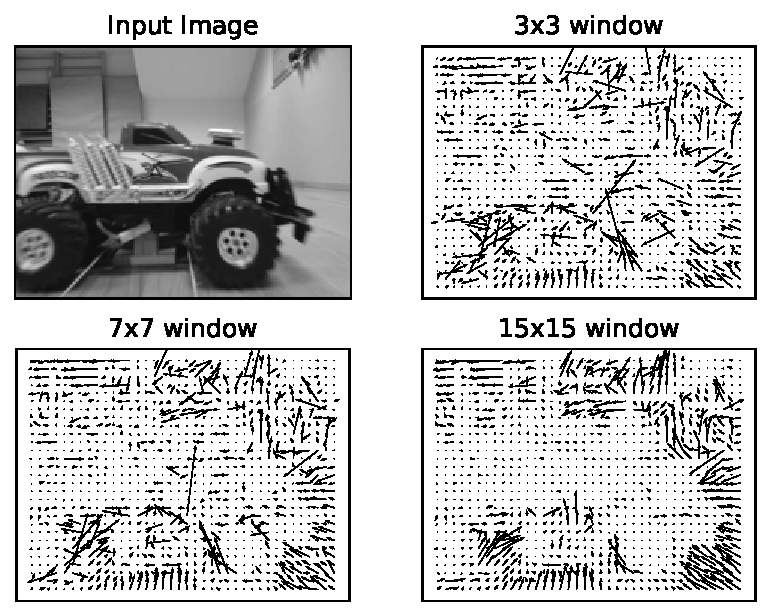
\includegraphics[width=0.5\textwidth]{LK_window.pdf}
    \vspace{-15px}
    \caption{Optical flow fields for Lucas-Kanade method with different window sizes.}
    \label{lk-window}
\end{figure}

Horn-Schunck method has two main parameters: the number of iterations $n$ and a regularization parameter $\lambda$ that affects the smoothness of the results.
The number of iterations $n$ determines how many times the method will iterate to minimize the energy of the flow field.
To determin a reasonable value $n$ we need to take into account computational expensiveness and the rate of convergence of $n$.
To stop unnecessary iterations we also implement a stopping criterion that stops the iterations when the change inthe flow field is smaller than e-8.
The effect of different number of iterations is shown in Figure \ref{hs-iterations}.

% Most of the difference can be seen in the lowe left corner wher the concentration of the flow vectors is the highest for $n$=100.
\begin{figure}[H]
    \centering
    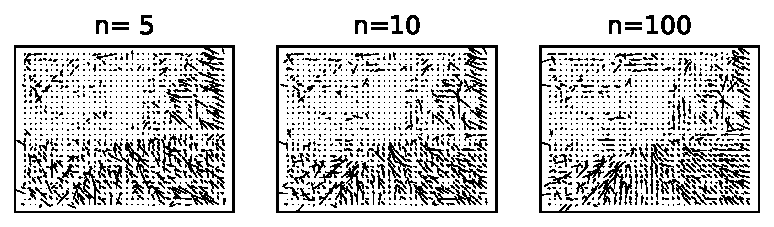
\includegraphics[width=0.5\textwidth]{HS_iter.pdf}
    \vspace{-15px}
    \caption{Optical flow fields for Horn-Schunck method with different number of iterations.}
    \label{hs-iterations}
\end{figure}

The regularization parameter $\lambda$ determines by how much we want to smooth the flow field as $\lambda$ increases the denominator of the equation becomes larger and thus smoothing the current flow vectors by a smaller amount.
Figure \ref{hs-lambda} shows the effect of $\lambda$ values of 0, 5 and 20. 
The biggest difference can be seen between $\lambda=0$ and other two values.
When $\lambda=0$ the values of the flow field are similar to raw derivatives and their directions are more noisy.
As $\lambda$ increases the flow field becomes smoother and better represents the motion in the image.
\begin{figure}[H]
    \centering
    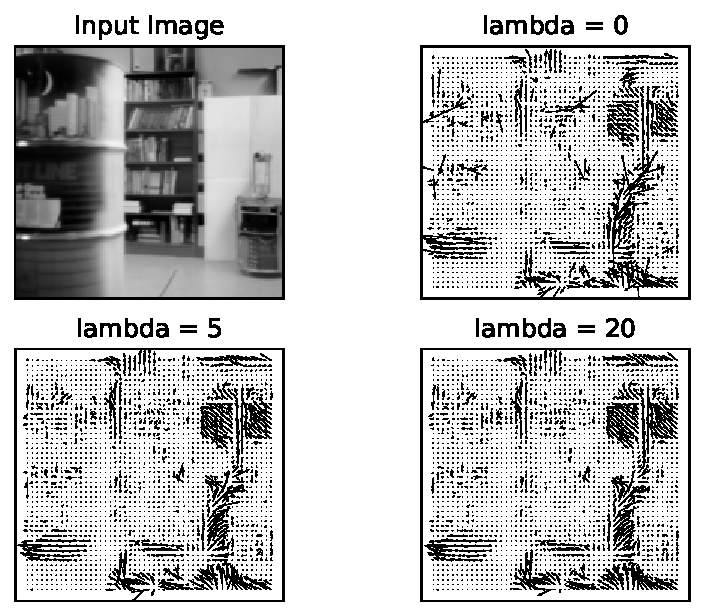
\includegraphics[width=0.5\textwidth]{HS_lambda.pdf}
    \vspace{-15px}
    \caption{Optical flow fields for Horn-Schunck method with different $\lambda$ values.}
    \label{hs-lambda}
\end{figure}

\subsection*{Speed comparison}
Implementation of these methods using standard for loops would greatly increase the computational time.
We use matrix operations and convolution to efficiently compute the optical flow fields.
In Table \ref{speed} we present the time it takes to compute the optical flow fields for both methods.
The Lucas-Kanade method is fasadasd ster than the Horn-Schunck method as it uses least squares to estimate the motion of the pixels.
The speed of the Horn-Schunck method is affected by the number of iterations.
For this reason we set the number of iterations at 10000 with a stopping criterion if the change in the flow field is smaller than e-8.
In the last row of Table \ref{speed} we show the speed of the Horn-Schunck method with Lucas-Kanade initialization.
Using the Lucas-Kanade initialization drops the computation time by 24\% down from an average speed of 16.3s to 12.4s.
\begin{table}[H]
    \centering
    \begin{tabular}{|c|c|}
        \hline
        Method & Time (s) \\
        \hline
        Lucas-Kanade & 0.01 \\
        Horn-Schunck & 16.3 \\
        Horn-Schunck (LK initialization) & 12.4 \\
        \hline
    \end{tabular}
    \caption{Computation times for Lucas-Kanade and Horn-Schunck methods.}
    \label{speed}

\end{table}

\section{Conclusion}
The Lucas-Kanade and Horn-Schunck methods are the most basic optical flow methods.
They work best for small motion in the image and without the implementation of pyramids they fail to estimate large motion.
In general the Horn-Schunck method is more robust and provides better results than the Lucas-Kanade method.

\bibliographystyle{IEEEtran}
\bibliography{bibliography}

\end{document}
